\documentclass[a4paper,11pt]{article}
\usepackage[english]{babel}
\usepackage{graphicx}
\usepackage{amsmath, amssymb}
\usepackage[colorlinks, linkcolor=black, anchorcolor=black, citecolor=black, urlcolor=black]{hyperref} % Hyperlink reference
\usepackage{natbib}
\bibpunct{(}{)}{;}{a}{}{,}

\graphicspath{{fig/}}

\newcommand{\dC}{$^{\circ}$C}
\newcommand{\dg}{$^{\circ}$}
\newcommand{\dN}{$^{\circ}$N}
\newcommand{\dS}{$^{\circ}$S}
\newcommand{\dW}{$^{\circ}$W}
\newcommand{\dE}{$^{\circ}$E}


\begin{document}

\vspace{2cm}
\pagestyle{empty}

{\Large{EUMETNET/ECSN optional programme:}}
\vspace{1cm}

{\Large{\textbf{'European Climate Assessment \& Dataset (ECA\&D)'}}}
\vspace{1cm}

{\Large{Algorithm Theoretical Basis Document (ATBD)}}
\vspace{10cm}

\begin{tabular}{l@{: }l}
Project number & EPJ029135\\
Author & Project team ECA\&D,\\
& Royal Netherlands Meteorological Institute KNMI\\
Date & \today \\
Version & 10.6\\
\end{tabular}

\newpage
\pagenumbering{arabic}
\pagestyle{plain}

\tableofcontents

\newpage

\section{Project description}

\subsection{Objectives}
\label{sec:obj}

The European Climate Assessment \& Dataset project (ECA\&D) started in
2003 as the follow-up to ECA (for which KNMI was responsible member
since 1998). Between 2003 and 2008 the project has been partially
funded by EUMETNET. From 2009 onwards, KNMI has committed itself to
fund ECA\&D.
ECA\&D has now obtained the status of Regional Climate Centre (RCC)
for high resolution observation data in WMO Region VI (Europe and
the Middle East). 

The objective of ECA\&D is to analyze the temperature and
precipitation climate of WMO region VI, with special focus on trends
in climatic extremes observed at meteorological stations. For this
purpose, a dataset of 20th-century daily surface air temperature and
precipitation series has been compiled \citep{kleintank2002} and
tested for homogeneity \citep{wijngaard}.

To enable periodic assessments of climate change on a European scale,
a sustainable system for data gathering, archiving, quality control,
analysis and dissemination has been realized. Data gathering refers to
long-term daily resolution climatic time series from meteorological
stations throughout Europe and the Mediterranean provided by
contributing parties (mostly National Meteorological Services (NMSs))
from over 40 countries. Most series cover at least the period
1946--now. Archiving refers to transformation of the series to
standardized formats and storage in a centralized relational database
system. Quality control uses fixed procedures to check the data and
attach quality and homogeneity flags. Analysis refers to the
calculation of (extremes) indices according to internationally agreed
procedures specified by the CCL/CLIVAR/JCOMM Expert Team on Climate
Change Detection and Indices (ETCCDI, {\tt
http://www.clivar.org/organization/etccdi/etccdi.php}). Finally,
dissemination refers to making available both the daily data
(including quality flags) and the indices results to users through a
dedicated website.

Recently, the necessary steps have been completed for an improved
operational ECA\&D system as the first implementation of a Regional
Climate Centre (RCC) functionality for high resolution observational
data and extremes indices in WMO Region VI. This implies that the
system has been made more sustainable/transparent and has been
embedded into KNMIs information infrastructure. This ensures ongoing
support, guarantees well-performing up-and-running services and
documentation, backup- and maintenance procedures.

\subsection{Users}
\label{sec:users}

Because of its daily resolution, the ECA dataset enables a variety of
climate studies, including detailed analyses of changes in the
occurrence of extremes in relation to changes in the mean. Web
statistics, personal contacts and references in numerous publications,
advice reports and applications show that ECA\&D serves many
users. Also the ECA\&D report ''Climate of Europe, assessment of
observed daily temperature and precipitation extremes''
\citep{kleintank2002b} and its successor ''Towards an operational
system for assessing observed changes in climate extremes''
\citep{engelen} have received much praise. The project is widely
recognized as an example of KNMIs leading European role in the area of
climate data exchange and research. For example, the EU-FP6 project
MILLENNIUM uses a subset of long-term climate series for paleo
studies.

\subsection{Requirements}
\label{sec:require}

\begin{enumerate}
\item Not all countries will be able to submit their contribution in a
      standardized format at regular time intervals. Therefore, the
      continuation of individual treatment of each participant is
      crucial for success. This implies that dedicated solutions
      should be developed for each data provider, with the level of
      automation dependent on the technical and manpower possibilities
      of the respective participants.
\item The data come with different use permissions. We are allowed to
      redistribute some series to the general public, whereas others
      are only for index calculation and use in the calculation of the 
      gridded data products. The system should allow for different permission flags.
\item Since there is always a time lag between the most recent data
      contributed by participants and the present date, the
      observations from SYNOP messages for the same or nearby stations
      that are transmitted through the Global Telecommunication System
      (GTS) should temporarily be used to fill the gap. Once the
      `official' series are available from the data providers in
      participating countries, the temporary SYNOP data should be
      replaced. Regular updates, using SYNOP data and readily available
      participant data (see \S~\ref{sec:data:design}) are on a monthly
      basis. Requesting updates from all data participants is done on a
      less frequent basis. Each update of the daily data will be followed
      by a recalculation of quality control scores, indices, climatology, trends and
      homogeneity. This is followed by a calculations of provisional
      gridded datafiles for precipitation and daily maximum, minimum and averaged
      temperature for the past month.
%     Available updates of data series should at least be
%     implemented every 6 month, with newly acquired daily datasets
%     issued and described, as well as indices results updated.
\item The minimum set of metadata for each series, which is required
      to judge the quality and representativeness of the observations,
      is described in \citet{aguilar}. Metadata information is
      important since not all station observations conform closely to
      the recommendations of instrumentation, exposure and siting
      which are given in the WMO-CIMO Guide. Moreover, the
      recommendations have changed over time. The minimum set of
      metadata should be stored along with the data series. Some of
      these metadata are used in the blending process.
\item The system should adopt and comply with (inter)nationally agreed
      standards as much as possible. This refers both to data format
      and database standards as well as metadata description
      standards.
\item A subset of the stations with ECA\&D series is part of the GCOS
      Surface Network (GSN). For some of these stations, the daily
      series are collated and archived also at the WMO World Data
      Center A in Asheville (U.S.A.). Discrepancies between the series
      in ECA\&D and those in GSN should be carefully monitored. Data
      series in GSN that are not part of ECA\&D will be
      copied. %Additional public data sources have become available
      %from EU projects, such as the IMPROVE book and CDROM
      \citep{camuffo}.
\item The ECA\&D website, as a dissemination tool for data and indices
      results, should be easily accessible and flexible for many
      users. Researchers and operational climatologists have very
      different requirements. The possibility of different interfaces
      should be explored ranging from bulk download to customizable
      queries through the data and indices results. Also the output
      formats on screen and print should be flexible providing reports
      in different layouts. The daily data should be available to
      users in different stages of processing. This means that the
      'raw' data files (as received from the participants, including
      explanatory e-mails) as well as the reformatted and
      quality-controlled data should be stored.
\item The European Environment Agency (EEA) relies on the extremes
      indices for its European state of the environment reports, which
      are issued at regular intervals and aim to support sustainable
      development \citep{eea}. Contacts with responsible authors at
      EEA have learned that they would prefer using up-to-date
      information also for their annual assessments in particular with
      respect to index anomaly maps for individual years.
\item The existence of copies of (subsets of the) ECA dataset
      elsewhere on the Internet in reformatted files should be
      discouraged. Already, STARDEX ({\tt
      http://www.cru.uea.ac.uk/projects/stardex/}), GDCN ({\tt
      http://lwf.ncdc.noaa.gov/oa/climate/research/gdcn/gdcn.html})
      and the Climate Explorer ({\tt http://climexp.knmi.nl/})
      extracted and published copies of the entire dataset. The
      problem is that these ad-hoc copies often stay without regular
      updates. To improve this situation, specific agreements with
      responsible persons should be reached so that the required
      subsets are delivered straight from the ECA\&D source or
      provided at the ECA\&D website.
\item In several WMO working groups, KNMI has indicated its
      willingness to offer help to other continents, in particular
      Africa and South America to run similar projects as ECA\&D. Part
      of this capacity building will consist of infrastructure (web)
      issues. KNMI is also involved in an Indonesia project where
      ECA\&D will provide the infrastructure for analysis and
      distribution of data. In addition, there is the intention to use
      the ECA\&D system of presenting index results for worldwide
      indices collected by the ETCCDI. To be prepared for these future
      requests, the developed system should keep into account such
      extensions.
\item The developed web interface should run easily on workstations
      and Internet PCs typically used in participating countries. This
      means that also lower capacity PCs (e.g. using MS Windows 95 on
      386 processor PCs with 8 Mb ram and 800x600 screen resolution
      with 256 colors and 56k modem) should be able to use the
      interface without difficulties. All popular web browsers should
      be supported (MS Internet Explorer, Netscape Navigator, Mozilla,
      Opera, Lynx). Performance of the system should meet minimum
      standards. For all parts of the user interface maximum waiting
      time (assuming optimum Internet speed and advanced PCs or
      workstations) should at maximum be in the order of 3 to 5
      seconds.
\item Operational guarantees for the system outside the KNMI firewall, which 
      has the website and database running, are on a 8/5 basis. 
      Bringing the system up and running again at the next
      working day is satisfactory, provided that 
      the archived data are in no danger.  User access monitoring facilities
      should be used to count the number of hits and to determine user
      preferences. This information is to be used primarily for
      further improvements of the system.
\item The technical solutions should benefit from the routine backup-
      and maintenance procedures KNMI employs. Optimal use should be
      made of KNMI information systems and infrastructure to ensure
      ongoing support and to guarantee up-and-running services from
      the ECA data\-base and website and to ensure restoring data, with
      no loss. Regular and reliable backup procedures should be
      maintained. On the other hand, changes in the KNMI
      infrastructure should not negatively affect the results of the
      ECA\&D project.
\end{enumerate}

\subsection{Infrastructure and software}
\label{sec:infra}

At the moment, two dedicated ECA\&D systems are in use: the develop \&
test environment and the operational system (outside the
firewall). All procedures are run on a developer platform and the
results are copied to the operational platform. The operating system
is Linux. The web-server is Apache. A functional controller, which is
embedded within KNMI's ICT infrastructure, permanently monitors the
performance of the operational system using the open source
software Nagios ({\tt http://www.nagios.org}). A MySQL
database is used to store the data and corresponding metadata. Most of
the software used to update the database are written in Bash, Fortran
and C code. More details about the infrastructure can be found in the
internal document about the ECA\&D infrastructure.
% which forms an Appendix to this ATBD.


\subsection{Data flow}
\label{sec:flow}

The necessary \underline{steps in data processing} are:
\begin{enumerate}
\item New data import
\item Quality control
\item Blending
\item Indices calculation
\item Climatology calculation
\item Trend calculation
\item Homogeneity analysis
\item E-OBS gridded dataset
\item Website
\end{enumerate}

For each step, the main method is described in the sections below. 
%More details can be found in the internal document describing the programs themselves.


\section{New data import}
\subsection{Design rules}
\label{sec:data:design}

Participant data comes in various file formats. Importing this data
into the database tables is entirely done by hand, running relevant
scripts to do the conversions. The conversions differ for each data
source. Dependent on the permissions granted by the data providers,
data series can either be: downloadable or
non-downloadable. Non-downloadable data are only used in the
calculation of the trends, indices and the gridded datasets, while the
downloadable data are published on the web as well. Most station
series are updated irregularly, each time after the data providers are
contacted.

A few stations are updated on a monthly basis. The stations in Norway
and Slovenia are updated via the data they provide on their
websites. For Dutch stations, a link is made with the Dutch
meteorological database. Luxembourg Airport is updated via monthly
emails send by the data provider of that station. Data for stations in
Germany and Czech Republic are provided every month by FTP.

The data provided by the participants is always received with some
delay. It is not possible for all of the participants to deliver
(near) real time data, because of validation and verification. To
update each series at the time that participant data has not yet
arrived, SYNOP messages are used. The source for these synoptical data
is the ECMWF MARS-archive (see
{\tt http://www.ecmwf.int/services/archive/}). This archive is a complete
and consistent representation of SYNOP messages distributed over the
GTS. Synoptical data is retrieved from the MARS-archive only for
WMO-Region VI and countries in North Africa. For technical reasons,
this is translated to be all land stations that fit in the rectangle
90N/40W and 10N/80E. Data retrieval is restricted to the reports of
the main hours 00, 06, 12 and 18 UT.

Daily minimum and maximum temperatures are reported at 6 UT and 18 UT 
respectively, and refer to the 12-hour periods preceding these points in time. 
These values therefore do not cover a full 24-hour period. 
The impact of this mismatch and issues related to the quality of the synoptical data
is currently under investigation.
%The impact of this mismatch and issues related to the quality of the synoptical data
%is addressed by \citet{vandenbesselaar:10}.

Daily values for the following 9 elements are derived from the SYNOP
messages:

\begin{description}
\item[Daily maximum temperature TX] In the synoptical report of 18
UT, the daily maximum temperature is given for that day. This daily
maximum temperature is the highest temperature recorded between 06 UT
and 18 UT (according to WMO specifications).
\item[Daily minimum temperature TN] In the synoptical report of 06 UT,
the daily minimum temperature is given for that day. This daily
minimum temperature is the lowest temperature recorded between 18 UT
(previous day) and 06 UT (according to WMO specifications).
\item[Daily mean temperature TG] If the daily maximum temperature (TX)
and the daily minimum temperature (TN) is known, mean daily
temperature is calculated as TG=(TX+TN)/2. This combines the TX reading 
of 18 UT and that of TN of 6 UT of the current day.
\item[Daily mean sea level pressure PP] Whenever sea level pressure
data is available at 00, 06, 12 and/or 18 UT, daily mean sea level
pressure is calculated as the average of the available values.
\item[Daily precipitation amount RR] Whenever synoptical 12-hourly
precipitation data is available at 06 and 18 UT, daily precipitation
is calculated as the sum of RR of 18UT of the current day and RR of 
6 UT of the next day.
\item[Daily mean snow depth SD] Whenever synoptical snow depth data is
available at 00, 06, 12 and/or 18 UT, daily mean snow depth is calculated
as the average snow depth of the available values.
\item[Daily mean cloud cover CC] Whenever synoptical cloud cover data
is available at 00, 06, 12 and/or 18 UT, mean daily cloud cover is
calculated as the average of the available values. This value in
percent is converted to octas by ROUND((cloud
cover\_in\_percents/100)*8).
\item[Sunshine duration SS] Whenever synoptical sunshine duration is
available (in minutes) at 00, 06, 12 and/or 18 UT, daily sunshine
duration is calculated as the summation of the available values.
\item[Daily mean humidity HU] Whenever synoptical humidity data is
available (in percents) at 00, 06, 12 and 18 UT, daily mean humidity is
calculated as the mean of the available values.
\item[Daily mean wind speed FG] Whenever synoptical wind speed data is
available (in m/s) at 00, 06, 12 and 18 UT, daily mean wind speed is
calculated as the mean of the available values.
\item[Daily maximum wind gust FX] Whenever synoptical wind gust data
is available (in m/s) at 00, 06, 12 and 18 UT, daily maximum wind gust
is taken as the maximum of the available values.
\item[Wind direction DD] Whenever synoptical wind direction data is
available (in degrees) at 12 UT, that value is taken as the wind
direction.
\end{description}

\subsection{Current implementation}
\label{sec:currentimpl}

Within the ECA\&D relational database, various types of tables are
distinguished: core tables that hold the unique raw data, working
tables that hold temporarily stored data and so-called derived tables
that hold derived data calculated according to the rules specified in
the remainder of this document. Derived data is updated by running the
various processes. It is necessary to store these derived data for
better performance of subsequent procedures and/or the website. Data
for different elements xx are stored in separate tables. Based on the
use permissions that participants have given to their data, two
different targets are distinguished. Likewise, tables have extensions
for the targets: public and mixed. \emph{Mixed} indicates downloadable
data combined with non-downloadable data. The data in the \emph{mixed}
tables are used for indices, trends and gridding, while only the data
in \emph{public} are available for download on the website. Data in
the \emph{public} tables are a subset of those in the \emph{mixed}
tables.

The SYNOP messages from the ECMWF MARS-archive are downloaded on a
monthly basis. The data archive comes in a BUFR-format, a WMO defined
format for irregular spaced point data. To process this BUFR-formatted
archive, the ECMWF BUFRDC subroutines are used. These subroutines
expand the BUFR-file into ASCII-readable data, which is processed
further. The subroutines extract only the data required, i.e. TX, TN,
PP, RR, SD, CC, HU and SS, corresponding respectively with BUFR-fields:\\
12014 (maximum temperature at 2 m, past 12 hours),\\
12015 (minimum temperature at 2 m, past 12 hours),\\ 
10051 (pressure reduced to mean sea level),\\
13022 (total precipitation past 12 hours),\\
13013 (total snow depth),\\
20010 (cloud cover (total)),\\
13003 (relative humidity),\\
14031 (total sunshine),\\
11011 (wind direction),\\
11012 (wind speed),\\
11041 (wind gust).\\

After extraction into a ASCII-formatted file, every TX, TN, PP, RR,
SD, CC, HU, SS, FG, FX and DD (and the calculated TG) of a synoptical
station is stored in a temporary table. When the complete ASCII-file
is processed, another process reads this temporary table and
determines the daily values. Details about the programs that do this,
can be found in an accompanying internal document.





\section{Quality control}
\label{sec:qc}

\subsection{Design rules}
\label{sec:qcrules}

Quality control (QC) procedures flag each individual observation in a
series. Separate QC procedures are performed for the station series
(non-blended) and the blended series.  Three QC flags are currently
implemented:

\begin{itemize}
\item Flag=0: 'valid'
\item Flag=1: 'suspect'
\item Flag=9: 'missing'
\end{itemize}

The following conditions apply for each element.
\medskip

\noindent{\textbf{daily precipitation amount RR:}}\\
\ldots must be equal or exceed 0 mm\\
\ldots must be less than 300.0 mm\\
\ldots must not be repetitive (i.e. exactly the same amount) for 10
days in a row if amount larger than 1.0 mm\\
\ldots must not be repetitive (i.e. exactly the same amount) for 5
days in a row if amount larger than 5.0 mm\\
\ldots dry periods receive flag = 1 (suspect), if the amount of dry
days lies outside a 14$\cdot$bivariate standard deviation
\medskip

\noindent{\textbf{daily mean surface air pressure PP:}}\\
\ldots must exceed 900.0 hPa\\
\ldots must be less than 1080.0 hPa\\
\ldots must not be repetitive (i.e. exactly the same) for 5 days in a row
\medskip

\noindent{\textbf{daily maximum temperature TX:}}\\
\ldots must exceed -90.0 $^{\circ}$C\\
\ldots must be less than 60.0 $^{\circ}$C\\
\ldots must exceed or equal daily minimum temperature (if exists)\\
\ldots must exceed or equal daily mean temperature (if exists)\\
\ldots must not be repetitive (i.e. exactly the same) for 5 days in a row\\
\ldots must be less than the long term average daily maximum
temperature for that calendar day + 5 times standard deviation
(calculated for a 5 day window centered on each calendar day over the
whole period)\\
\ldots must exceed the long term average daily maximum temperature for
that calendar day - 5 times standard deviation (calculated for a 5 day
window centered on each calendar day over the whole period)
\medskip

\noindent{\textbf{Daily minimum temperature TN:}}\\
\ldots must exceed -90.0 $^{\circ}$C\\
\ldots must be less than 60.0 $^{\circ}$C\\
\ldots must be less or equal to daily maximum temperature (if exists)\\
\ldots must be less or equal to daily mean temperature (if exists)\\
\ldots must not be repetitive (i.e. exactly the same) for 5 days in a row\\
\ldots must be less than the long term average daily minimum
temperature for that calendar day + 5 times standard deviation
(calculated for a 5 day window centered on each calendar day over the
whole period)\\
\ldots must exceed the long term average daily minimum temperature for
that calendar day - 5 times standard deviation (calculated for a 5 day
window centered on each calendar day over the whole period)
\medskip

\noindent{\textbf{Daily mean temperature TG:}}\\
\ldots must exceed -90.0 $^{\circ}$C\\
\ldots must be less than 60.0 $^{\circ}$C\\
\ldots must exceed or equal daily minimum temperature (if exists)\\
\ldots must be less or equal to daily maximum temperature (if exists)\\
\ldots must not be repetitive (i.e. exactly the same) for 5 days in a row\\
\ldots must be less than the long term average daily mean temperature
for that calendar day + 5 times standard deviation (calculated for a 5
day window centered on each calendar day over the whole period)\\
\ldots must exceed the long term average daily mean temperature for
that calendar day - 5 times standard deviation (calculated for a 5 day
window centered on each calendar day over the whole period)
\medskip

\noindent{\textbf{Daily snow depth SD:}}\\
\ldots must exceed or equal 0.0 cm\\
\ldots must be less than 300.0 cm if station elevation is less or equal to 400 m\\
\ldots must be less than 800.0 cm if station elevation is between 400 m and 2000 m\\
\ldots must be less than 1500.0 cm if station elevation is equal to or more than 2000 m
\medskip

\noindent{\textbf{Daily cloud cover CC:}}\\
\ldots must exceed or equal 0\\
\ldots must be less than or equal 8
\medskip

\noindent{\textbf{Daily humidity HU:}}\\
\ldots must exceed or equal 0.0\%\\
\ldots must be less than or equal to 100.0\%
\medskip

\noindent{\textbf{Daily sunshine duration SS:}}\\
\ldots must exceed or equal 0.0 h\\
\ldots must be less than 24.0 h
\medskip

\noindent{\textbf{Daily mean wind speed FG:}}\\
\ldots must exceed or equal 0.0 m/s\\
\ldots must be less than or equal to 46 m/s\\
\ldots must not be repetitive (i.e. exactly the same value) for 6
days in a row if value larger or equal to 2.0 m/s
\medskip

\noindent{\textbf{Daily maximum wind gust FX:}}\\
\ldots must exceed or equal 0.0 m/s\\
\ldots must be less than or equal to 76 m/s\\
\ldots must not be repetitive (i.e. exactly the same value) for 5
days in a row if value larger or equal to 4.0 m/s
\medskip

\noindent{\textbf{Daily mean wind direction DD:}}\\
\ldots must exceed or equal 0.0 degrees\\
\ldots must be less than or equal to 360 degrees\\
\ldots must not be repetitive (i.e. exactly the same value) for 6 days
in a row if value larger than 0.5 degrees
\medskip

The default QC flag is 0 ('valid'). If one of the conditions above is
not met: a QC flag of 1 ('suspect') is assigned. If data is missing:
QC=9 ('missing'). The conditions are tested in an automated procedure,
but a manual intervention is possible for non-blended series and the
manual QC flag will be propagated to the blended series. For instance,
precipitation extremes flagged 'suspect' are overruled if
supplementary evidence exists (e.g. from radar images or weather
charts) that the particular extreme is plausible.

If for a calendar day 10 or more samples exist, then the long-term
average or standard deviation is calculated for that day. In order to
adjust the day-to-day variability associated with the sampling, the
long-term averages are smoothed. The (smoothed) long-term average is
only calculated if the total number of days present is 25 or more. If
a calendar day does not meet these requirements (e.g. for a leap day),
the quality checks associated with long term averages are not
performed for that day.

\section{Blending}
\label{sec:blending}

\subsection{Design rules}
\label{sec:blendrules}

The procedure to calculate the optimal combination of ECA station and
nearby station (which can be an ECA station or a synoptical station)
has the following steps (applying spherical trigonometry):

\begin{enumerate}
\item Convert LAT and LON into decimal degrees. E.g. for station De
  Bilt this yields\\ 
\medskip

\begin{tabular}{l l l l}
Latitude:& 52:06N & LAT$_{\textrm{ECA}}$ &= 52+6/60 = 52.10\\
Longitude: &05:11E & LON$_{\textrm{ECA}}$ &= 5+11/60 = 5.18
\end{tabular}
\medskip

\item For every other station, also convert LAT and LON into decimal
degrees\\
\medskip

\begin{tabular}{l l l l}
Latitude: & HH$_{\textrm{LA}}$:MM$_{\textrm{LA}}$ &
LAT$_{\textrm{OTHER}}$ &= HH$_{\textrm{LA}}$+MM$_{\textrm{LA}}$/60\\
Longitude:& HH$_{\textrm{LO}}$:MM$_{\textrm{LO}}$ &
LON$_{\textrm{OTHER}}$ &= HH$_{\textrm{LO}}$+MM$_{\textrm{LO}}$/60
\end{tabular}
\medskip

If Latitude on southern hemisphere: LAT$_{\textrm{OTHER}}$ = -1 $\cdot$
LAT$_{\textrm{OTHER}}$\\
If Longitude on western hemisphere: LON$_{\textrm{OTHER}}$ = -1 $\cdot$ LON$_{\textrm{OTHER}}$
\medskip

\item Find a combination ECA-OTHER station by minimizing the distance
(here in km):
\medskip

 distance = radius\_earth $\times$
ARCCOS(SIN(atan$\cdot$LAT$_{\textrm{ECA}}$) $\times$
SIN(atan $\cdot$ LAT$_{\textrm{OTHER}}$) +
COS(atan $\cdot$ LAT$_{\textrm{ECA}}$) $\times$
COS(atan $\cdot$ LAT$_{\textrm{OTHER}}$) $\times$
COS(atan $\cdot$ (LON$_{\textrm{OTHER}}$ - LON$_{\textrm{ECA}}$)))\\
where: radius\_earth = 6378.137 kilometers, and atan = ARCTAN(1)/45
\medskip

Substituting for De Bilt, with LAT/LON from WMO synoptical or
ECA-stations yields:
\medskip

distance = radius\_earth $\times$
ARCCOS(SIN(atan $\cdot$ 52.10) $\times$
SIN(atan $\cdot$ LAT$_{\textrm{OTHER}}$) + COS(atan $\cdot$ 52.10) $\times$
COS(atan $\cdot$ LAT$_{\textrm{OTHER}}$) $\times$
COS(atan $\cdot$ (LON$_{\textrm{OTHER}}$ - 5.18)))
\medskip

Repeat distance for every OTHER station, keeping LAT$_{\textrm{ECA}}$
and LON$_{\textrm{ECA}}$ fixed (in the example above, for De
Bilt). The OTHER station with lowest distance is the station that is
nearest to De Bilt (in this example). Only data from stations that are
no more than 12.5 km away from the original ECA station, is used.

\item As a last step, the difference in elevation of the ECA station
  and OTHER station is considered. Only data from stations located
  within 25 m height difference is taken into account.
\end{enumerate}

Next, the blended series are constructed. Suppose we have a station
series from 1900 until 2005, with missing data between 1930 and 1935
and also after 2005. Now that we know what other stations are nearby
we are considering the data from these stations to 'infill' the gaps
or data values that are flagged as suspect during QC (as illustrated
in the figure below; see also Sect.~\ref{sec:qc}).

\begin{figure}[!ht]
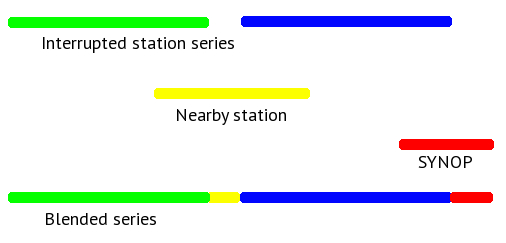
\includegraphics[width=\textwidth]{blended_fig_new1.jpg}
\caption{Blending figure}
\label{fig:blend}
\end{figure}

The logic that is applied when constructing the blended series is as
follows. First, valid data from nearby ECA stations is taken to
'infill' the gaps, i.e. days with qc=1 or missing data. If no valid
data from nearby ECA stations is available, valid data from nearby
synoptical stations is taken to 'infill' the gaps. If there is less
than 10 years difference between the year of the last date of the
series and the current date, the series are extended with synop data
from nearby synoptical stations as well. More details about the
blending process can be found in the accompanying internal document.

\section{Indices calculation}
\label{sec:indices}

\subsection{Design rules}
\label{sec:indicesrules}

Indices are calculated for the \emph{mixed} blended series only and
over a time span which is as long as the record allows.
For an index to be calculated for a
particular year, at least 350 days with valid daily data must
exist. For an index to be calculated for a half-year period, at least
175 days with valid daily data must exist. For an index to be
calculated for a seasonal period, at least 85 days with valid daily
data must exist. For an index to be
calculated for a monthly period, at least 25 days with valid daily
data must exist. Indices results are stored in the database only if a
series contains at least 10 years of valid data. 

A total of 61 indices are calculated on the basis of the blended daily
series for the categories Cold, Drought, Heat, Pressure, Rain, Snow,
Sunshine, Temperature, Wind and Compound. The acronyms are: 
 TG, TN, TX, DTR*, ETR, GD4, GSL*, vDTR, CFD, FD*, HD17, ID*, CSDI*, TG10p, TN10p*, TX10p*, SU*, TR*,
 WSDI*, TG90p, TN90p*, TX90p*, RR*, RR1, SDII*, CDD, CWD*, R10mm*, R20mm*, RX1day*, RX5day*, R75p, R75pTOT,
 R95p, R95pTOT*, R99p, R99pTOT*, PP, SPI3, SPI6, SD, SS, TXx*, TNx*, TXn*, TNn*, SSp, PET, SD1, SD5cm, SD50cm,
 CD, CW, WD, WW, CSU, RH, CC, CC2, CC6, PRCPTOT
%WIND:, FXx, FG6Bft, FGcalm, FG, WGF, DDnorth, DDsouth, DDwest, DDeast. 
Those with * are part of the ETCCDI list of 27 worldwide indices
available from {\tt http://cccma.seos. uvic.ca/ETCCDI/indices.shtml}.


The exact definition of each index is given in the next sections. Each
index is calculated as annual , winter half-year (ONDJFM), summer
half-year (AMJJAS), winter (DJF), spring (MAM), summer (JJA), autumn
(SON) and monthly values.

\subsection{Calculation of percentiles}
\citet{zhang:05} brought to the attention that 
percentiles, calculated on the basis of data from a `base'-period of the record, and subsequently applied
to data from the `out-of-base' period, will introduce inhomogeneities in the resulting exceedance series.
The inhomogeneities are strongest for high percentiles and for data with strong auto correlation.

In their article, they offer an alternative way to calculate percentiles when they are applied to the
base-period. This method of calculating percentiles is adopted by ECA\&D. This procedure is:~\citep[\S 4]{zhang:05}
\begin{enumerate}
\item The 30-yr base period is divided into one `out of base' year, the year for which exceedance is to be estimated,
and a `base period' consisting of the remaining 29 yr from which the thresholds would be estimated.
\item A 30-yr block of data is constructed by using the 29-yr base period dataset and adding an additional
year of data from the base period (replicating one year in the base period). This constructed 30-yr block
 is used to estimate thresholds. 
\item The out-of-base year is then compared with these thresholds, and the exceedance rate for the out-of-base year is obtained.
\item Steps 2 and 3 are repeated an additional 28 times, by repeating each of the remaining 28 in-base years in turn
to construct the 30-yr block.
\item The final index for the out-of-base year is obtained by averaging the 29 estimates obtained from steps 2, 3 and 4.
\end{enumerate}

\subsection{Smoothing of indices}
Next to the actual index values, smoothed index values are provided based on the application of a LOWESS 
(locally weighted scatterplot smoothing) smoother. This smoother fits simple models to localized subsets 
of the data to build up a function that describes the deterministic part of the variation in the data, point by point.

The code is based on routines provided by W. S. Cleveland (Bell Laboratories, Murray Hill NJ).

The smoother span $f$ gives the proportion of points in the plot which influence
the smooth at each value. The value of $f$ is set to:
\begin{equation*}
f = {30 \over \text{length of record in years}}.
\end{equation*}
This gives higher values for $f$ when the length of the series is short, giving more smoothness.

The number of `robustifying' iterations which should be performed is set to 3.

The parameter $\delta$ is used to speed up computation: instead of computing the local polynomial fit at each data
point it is not computed for points within $\delta$ of the last computed point, and linear interpolation
is used to fill in the fitted values for the skipped points.
This parameter is set to 1/100th of the range of the input data, which is generally regarded as a standard value.

\subsubsection{Cloudiness indices}

\subsection*{CC}
\begin{itemize}
\item \textit{Mean of daily cloud cover (oktas)}
\end{itemize}
Let $CC_{ij}$ be the daily cloud cover at day $i$ of period
$j$. Then mean values in period $j$ are given by:
\begin{equation*}
CC_{j} = \frac{\sum_{i=1}^{I} CC_{ij}}{I}
\end{equation*}

\subsection*{CC2}
\begin{itemize}
\item \textit{Mostly sunny days (cloud cover $\leq$ 2 oktas) (days)}
\end{itemize}
Let $CC_{ij}$ be the daily cloud cover at day $i$ of period
$j$. Then counted is the number of days where:
\begin{equation*}
CC_{ij} \leq 2 \:oktas
\end{equation*}

\subsection*{CC6}
\begin{itemize}
\item \textit{Mostly cloudy days (cloud cover $\geq$ 6 oktas) (days)}
\end{itemize}
Let $CC_{ij}$ be the daily cloud cover at day $i$ of period
$j$. Then counted is the number of days where:
\begin{equation*}
CC_{ij} \geq 6 \:oktas
\end{equation*}


\subsubsection{Cold indices}

\subsection*{GD4}
\begin{itemize}
\item \textit{Growing degree days (sum of TG $>$ $4$ $^\circ$C)
($^\circ$C)}
\end{itemize}
Let $TG_{ij}$ be the daily mean temperature at day $i$ of period
$j$. Then the growing degree days are:
\begin{equation*}
GD4_{j} = \sum_{i=1}^{I}(TG_{ij}-4 \mid TG_{ij} > 4 \:^{\circ}C)
\end{equation*}

\subsection*{GSL}
\begin{itemize}
\item \textit{Growing season length (days)}
\end{itemize}
Let $TG_{ij}$ be the mean temperature at day $i$ of period $j$. Then
counted is the number of days between the first occurrence of at least 6
consecutive days with:
\begin{equation*}
TG_{ij} > 5 \:^\circ C
\end{equation*}
and the first occurrence after 1 July of at least 6 consecutive days
with: 
\begin{equation*}
TG_{ij} < 5 \:^\circ C
\end{equation*}

\subsection*{HI}
\begin{itemize}
\item \textit{Huglin Index}
\end{itemize}
The Huglin Index is an index specifically aimed at grap growth~\citep{huglin:78} and defined 
using daily averaged temperature $t_g$ and the daily maximum
temperature $t_x$ for the period 1 April to 30 September:
\begin{equation}
HI = \sum_{01/04}^{30/09} {(tg - 10) + (tx - 10) \over 2} K \notag
\end{equation}
where $K$ is a daylength coefficient. The daylight coefficient is a function of the latitude of the station
but a  clear definition is absent. The value of $K$ is determined using table~\ref{table:daylightcoef}.

\begin{table} [!h]
\begin{tabular}{l l}
latitude  & daylight coefficient $K$ \\
\hline
$\le$ 40\dN & 1.00 \\
40\dN-42\dN & 1.02 \\
42\dN-44\dN & 1.03 \\
44\dN-46\dN & 1.04 \\
46\dN-48\dN & 1.05 \\
48\dN-50\dN & 1.06 \\
\end{tabular}
\caption{The daylight coefficient as used in the Huglin index as a function of latitude.
} \label{table:daylightcoef}
\end{table}

\subsection*{BEDD}
\begin{itemize}
\item \textit{Biologically Effective Degree Days}
\end{itemize}
The Biologically Effective Degree Days index has been specifically targeted to describe grape 
growth~\citep{gladstones:92}.
The BEDD index is based on the Growing Degree Days
\begin{equation}
GDD_i= \text{max} \left[ \left({t_x + t_n \over 2} \right) -b, 0 \right], \notag
\end{equation}
where $b = 10$ is an appropriate value for grape growth.
The BEDD is calculated subsequently by 
\begin{equation}
BEDD = \sum_{01/04}^{30/09} \text{min} \left[ GDD_i, 9 \right]. \notag
\end{equation}


\subsection*{CFD}
\begin{itemize}
\item \textit{Maximum number of consecutive frost days (TN $< 0^\circ$C) (days)}
\end{itemize}
Let $TN_{ij}$ be the daily minimum temperature at day $i$ of period
$j$. Then counted is the largest number of consecutive days where:
\begin{equation*}
TN_{ij} < 0 \:^\circ C
\end{equation*}

\subsection*{FD}
\begin{itemize}
\item \textit{Frost days (TN $< 0^\circ$C) (days)}
\end{itemize}
Let $TN_{ij}$ be the daily minimum temperature at day $i$ of period
$j$. Then counted is the number of days where:
\begin{equation*}
TN_{ij} < 0 \:^\circ C
\end{equation*}

\subsection*{HD17}
\begin{itemize}
\item \textit{Heating degree days (sum of $17$ $^\circ$C - TG)
($^\circ$C)}
\end{itemize}
Let $TG_{ij}$ be the daily mean temperature at day $i$ of period
$j$. Then the heating degree days are:
\begin{equation*}
HD17_{j} = \sum_{i=1}^{I}(17 \:^\circ C - TG_{ij})
\end{equation*}

\subsection*{ID}
\begin{itemize}
\item \textit{Ice days (TX $< 0^\circ$C) (days)}
\end{itemize}
Let $TX_{ij}$ be the daily maximum temperature at day $i$ of period
$j$. Then counted is the number of days where:
\begin{equation*}
TX_{ij} < 0\: ^\circ C
\end{equation*}


\subsection*{CSDI}
\begin{itemize}
\item \textit{Cold-spell duration index (days)}
\end{itemize}
Let $TN_{ij}$ be the daily minimum temperature at day $i$ of period
$j$ and let $TN_{in}10$ be the calendar day 10th percentile calculated
for a 5-day window centred on each calendar day in the 1961--1990
period. Then counted is the number of days per period where, in
intervals of at least 6 consecutive days:
\begin{equation*}
TN_{ij} < TN_{in}10
\end{equation*}

\subsection*{TG10p}
\begin{itemize}
\item \textit{Days with TG $<$ 10th percentile of daily mean temperature
(cold days) (days)}
\end{itemize}
Let $TG_{ij}$ be the daily mean temperature at day $i$ of period $j$
and let $TG_{in}10$ be the calendar day 10th percentile calculated for
a 5-day window centred on each calendar day in the 1961--1990
period. Then counted is the number of days where:
\begin{equation*}
TG_{ij} < TG_{in}10
\end{equation*}

\subsection*{TN10p}
\begin{itemize}
\item \textit{Days with TN $<$ 10th percentile of daily minimum
temperature (cold nights) (days)}
\end{itemize}
Let $TN_{ij}$ be the daily minimum temperature at day $i$ of period
$j$ and let $TN_{in}10$ be the calendar day 10th percentile calculated
for a 5-day window centred on each calendar day in the 1961--1990
period. Then counted is the number of days where:
\begin{equation*}
TN_{ij} < TN_{in}10
\end{equation*}

\subsection*{TX10p}
\begin{itemize}
\item \textit{Days with TX $<$ 10th percentile of daily maximum
temperature (cold day-times) (days)}
\end{itemize}
Let $TX_{ij}$ be the daily maximum temperature at day $i$ of period
$j$ and let $TX_{in}10$ be the calendar day 10th percentile calculated
for a 5-day window centred on each calendar day in the 1961--1990
period. Then counted is the number of days where:
\begin{equation*}
TX_{ij} < TX_{in}10
\end{equation*}

\subsection*{TXn}
\begin{itemize}
\item \textit{Minimum value of daily maximum temperature ($^\circ$ C)}
\end{itemize}
Let $TX_{ij}$ be the daily maximum temperature on day $i$ of period
$j$. Then the minimum daily maximum temperature for period $j$ is:
\begin{equation*}
TXn_{j} = min(TX_{ij})
\end{equation*}

\subsection*{TNn}
\begin{itemize}
\item \textit{Minimum value of daily minimum temperature ($^\circ$ C)}
\end{itemize}
Let $TN_{ij}$ be the daily minimum temperature on day $i$ of period
$j$. Then the minimum daily minimum temperature for period $j$ is:
\begin{equation*}
TNn_{j} = min(TN_{ij})
\end{equation*}

\subsubsection{Compound indices}

The indices CD, CW, WD, and WW are based on \citet{beniston}.

\subsection*{CD}
\begin{itemize}
\item \textit{Days with TG $<$ 25th percentile and RR $<$ 25th percentile (cold/dry)}
\end{itemize}
Let $TG_{ij}$ be the daily mean temperature at day $i$ of period $j$
and let $TG_{in}25$ be the calendar day 25th percentile calculated for
a 5-day window centred on each calendar day in the 1961--1990
period. Let $RR_{wj}$ be the daily precipitation amount at wet day $w$
($RR\geq1.0$ mm) of period $j$ and let $RR_{wn}25$ be the 25th
percentile of precipitation at wet days in the 1961--1990 period. Then
counted is the number of days where:
\begin{equation*}
TG_{ij} < TG_{in}25 \qquad \textrm{and} \qquad RR_{wj} < RR_{wn}25
\end{equation*}

\subsection*{CW}
\begin{itemize}
\item \textit{Days with TG $<$ 25th percentile and RR $>$ 75th percentile (cold/wet)}
\end{itemize}
Let $TG_{ij}$ be the daily mean temperature at day $i$ of period $j$
and let $TG_{in}25$ be the calendar day 25th percentile calculated for
a 5-day window centred on each calendar day in the 1961--1990
period. Let $RR_{wj}$ be the daily precipitation amount at wet day $w$
($RR\geq1.0$ mm) of period $j$ and let $RR_{wn}75$ be the 75th
percentile of precipitation at wet days in the 1961--1990 period. Then
counted is the number of days where:
\begin{equation*}
TG_{ij} < TG_{in}25 \qquad \textrm{and} \qquad RR_{wj} > RR_{wn}75
\end{equation*}

\subsection*{WD}
\begin{itemize}
\item \textit{Days with TG $>$ 75th percentile and RR $<$ 25th percentile (warm/dry)}
\end{itemize}
Let $TG_{ij}$ be the daily mean temperature at day $i$ of period $j$
and let $TG_{in}75$ be the calendar day 75th percentile calculated for
a 5-day window centred on each calendar day in the 1961--1990
period. Let $RR_{wj}$ be the daily precipitation amount at wet day $w$
($RR\geq1.0$ mm) of period $j$ and let $RR_{wn}25$ be the 25th
percentile of precipitation at wet days in the 1961--1990 period. Then
counted is the number of days where:
\begin{equation*}
TG_{ij} > TG_{in}75 \qquad \textrm{and} \qquad RR_{wj} < RR_{wn}25
\end{equation*}

\subsection*{WW}
\begin{itemize}
\item \textit{Days with TG $>$ 75th percentile and RR $>$ 75th percentile (warm/wet)}
\end{itemize}
Let $TG_{ij}$ be the daily mean temperature at day $i$ of period $j$
and let $TG_{in}75$ be the calendar day 75th percentile calculated for
a 5-day window centred on each calendar day in the 1961--1990
period. Let $RR_{wj}$ be the daily precipitation amount at wet day $w$
($RR\geq1.0$ mm) of period $j$ and let $RR_{wn}75$ be the 75th
percentile of precipitation at wet days in the 1961--1990 period. Then
counted is the number of days where:
\begin{equation*}
TG_{ij} > TG_{in}75 \qquad \textrm{and} \qquad RR_{wj} > RR_{wn}75
\end{equation*}

\subsection*{UTCI}
\begin{itemize}
\item \textit{Mean of the Universal Thermal Climate Index}
\end{itemize}

The assessment of the thermophysiological effects of the atmospheric environment is one of the key issues in
human biometeorology. To quantify these effect, the Universal Thermal Climate Index (UTCI) is developed
in COST action 730. 

Input to the UTCI are mean radiant temperature, air temperature, water vapour 
pressure and windspeed.
The algorithm for the mean radiant temperature is the one given by~\citet{fanger:70}. Documentation for
the mean radiant temperature and the UTCI is available via http://www.utci.org.

In ECA\&D, data for daily averaged windspeed, relative humidity and sunshine duration are available which
we will use as input for calculating the mean radiant temperature and the UTCI. For this purpose, sunshine 
duration is related to an estimate of direct solar radiation (which is required as input to the mean radiant
temperature) and relative humidity is related to 
water vapour pressure using values of the daily maximum and minimum temperatures. The algorithms used for
these conversions are documented elsewhere~\citet{allen:94a,allen:94b,duffie:91}.

Since the UTCI relates to human activity, we use the daily
\emph{maximum} temperature as the air temperature since we can expect outdoor human activity to occur
during the day time.

In the mean radiant temperature, the projected area factor $f_g$ is included
which is related to the angle of the sun. Again since outdoor activity is in the day time, we take the
average of $f_g$ over the period 10:00h to 20:00h.

\subsection*{TCI}
\begin{itemize}
\item \textit{Mean of the Tourism Climatic Index}
\end{itemize}
The Tourism Climatic Index (TCI) represents a quantitative evaluation
of world climate for the purposes of tourism and is a composit
measure of the climatic well-being of tourists. 
The TCI is aimed at the tourists involved in site-seeing or light outdoors activities. 
The TCI is originally defined by~\citet{mieczkowski:85} as a weighted sum of several factors:
\begin{equation} \label{eq:tci1}
\text{TCI} = 2 \left( 4 \text{CI}_d + \text{CI}_a + 2 \text{R} + 2 \text{S} + W \right) \notag
\end{equation}
with CI$_d$ the daytime Comfort Index, CI$_a$ the daily Comfort Index, R the monthly precipitation sum,
S the average daily sunshine duration and W the average windspeed. 

The value of the TCI vary between 100 (`Ideal') to $<$10 (`Impossible'). The rating categories of the
Tourism Climatic Index are shown in Table~\ref{table:TCI}.

\citet{mieczkowski:85} defines tables which relate the various inputs to the TCI (eq.~\ref{eq:tci1}) to
climatic parameters. These discrete relations are interpolated using a chebyshev approximation to yield
a continuous relation between daily climate data and the TCI. 

\citet{mieczkowski:85} uses a thermal comfort rating based on the effective temperature as
calculated by the American Society of Heating, Refrigerating and Air Conditioning Engineers~\citep{ashrae:72},
and~\citet{mieczkowski:85} has translated
the effective temperature in a rather ad-hoc fashion to the thermal comfort rating. The relation
between temperature and humidity leading to the thermal comfort rating is captured in a simple
look-up table.

The relation between precipitation, daily sunshine duration and wind are given by ~\citet{mieczkowski:85}. 
Following~\citet{perch-nielsen:10}, the latter input has been modified. The `wind chill index' 
used orginally appeared to be seriously flawed and is replaced by the wind chill equivalent temperatures
defined by~\citet{osczevski:05}.

\begin{table} [!h]
\begin{tabular}{l l}
TCI & description \\
\hline
90-100 & ideal \\
80-89  & excellent \\
70-79  & very good \\
60-69  & good \\
50-59  & acceptable \\
40-49  & marginal \\
30-39  & unfavourable \\
20-29  & very unfavourable \\
10-19  & extremely unfavourable \\
$<$10  & impossible \\
\end{tabular}
\caption{A classification scheme for the Tourism Climatic Index.
} \label{table:TCI}
\end{table}



\subsection*{TCI60}
\begin{itemize}
\item \textit{Days where the Tourism Climatic Index $\ge$ 60}
\end{itemize}
The Tourism Climatic Index (TCI) represents a quantitative evaluation
of world climate for the purposes of tourism and is a composit
measure of the climatic well-being of tourists. 

Let TCI$_{ij}$ be the daily value of the Tourism Climatic Index at day $i$ of period $j$.
Then counted is the number of days where:
\begin{equation*}
\text{TCI}_{ij} \ge 60
\end{equation*}
The value TCI=60 represents the lowest level where the climatic conditions for sight-seeing or light outdoors
activities following the classification of the Tourism Climatic Index is `good'.


\subsection*{TCI80}
\begin{itemize}
\item \textit{Days where the Tourism Climatic Index $\ge$ 80}
\end{itemize}
The Tourism Climatic Index (TCI) represents a quantitative evaluation
of world climate for the purposes of tourism and is a composit
measure of the climatic well-being of tourists. 

Let TCI$_{ij}$ be the daily value of the Tourism Climatic Index at day $i$ of period $j$.
Then counted is the number of days where:
\begin{equation*}
\text{TCI}_{ij} \ge 80
\end{equation*}
The value TCI=80 represents the lowest level where the climatic conditions for sight-seeing or light outdoors
activities following the classification of the Tourism Climatic Index is `excellent'.

\subsubsection{Drought indices}

\subsection*{CDD}
\begin{itemize}
\item \textit{Maximum number of consecutive dry days (RR $<$ 1 mm) (days)}
\end{itemize}
Let $RR_{ij}$ be the daily precipitation amount for day $i$ of period
$j$. Then counted is the largest number of consecutive days where:
\begin{equation*}
RR_{ij} < 1~mm
\end{equation*}

\subsection*{SPI6}
\begin{itemize}
\item \textit{6-Month Standardized Precipitation Index}
\end{itemize}
SPI is a probability index based on precipitation. It is designed to
be a spatially invariant indicator of drought. SPI6 refers to
precipiation in the previous 6-month period (+ indicates wet; -
indices dry).

See for details and the algorithm: \citet{guttman:99}.

\subsection*{SPI3}
\begin{itemize}
\item \textit{3-Month Standardized Precipitation Index}
\end{itemize}
SPI is a probability index based on precipitation. It is designed to
be a spatially invariant indicator of drought. SPI3 refers to
precipiation in the previous 3-month period (+ indicates wet; -
indices dry).

See for details and the algorithm: \citet{guttman:99}.

\subsection*{PET}
\begin{itemize}
\item \textit{Potential EvapoTranspiration}
\end{itemize}
PET is an index which gives the FAO-endorsed potential evapotranspiration
as calculated by the Penman-Monteith parametrization. 
Here reference crop evapotranspiration is a measure for potential evapotranspiration.
Reference crop evaporation is defined as the rate of evaporation from an
idealized grass reference crop with a fixed crop height of 0.12 m, an albedo of 0.23, and
a surface resistance of 70 s m$^{-1}$. In terms of of its evaporation rate, such a crop closely resembles
the reference crop of an extensive surface of short green grass cover of uniform height,
actively growing, completely shading the ground, and not short of water.

The equation used for estimating the reference crop evaporation is based on the Penman-Monteith approach;
\begin{equation}
ET_0 = {0.408 \Delta (R_n - G) + \gamma {900 \over T + 273} U_2 ( ea - e_d) \over
\Delta + \gamma ( 1 + 0.34 U_2) } \notag
\end{equation}
where\\
$ET_0$ : reference crop evapotranspiration\\
$R_n$ : net radiation at crop surface (using ECA\&D elements: sunshine duration and cloud cover)\\
$G$ : soil heat flux (using ECA\&D element: daily averaged temperature)\\
$T$ : daily averaged temperature\\
$U_2$ : daily averaged windspeed at 2 m height (using ECA\&D element: daily averaged wind speed at 10 m)\\
$(e_a - e_d)$ : vapour pressure deficit (using ECA\&D elements: relative humidity and daily averaged temperature) \\
$\Delta$ : slope vapour pressure (using ECA\&D element: daily averaged temperature)\\
$\gamma$ : psychrometric constant (using ECA\&D element: daily averaged sea-level pressure)\\
$900$ : coefficient for the reference crop\\
$0.34$ : wind coefficient for the reference crop\\
This equation is referred to as the FAO Penman-Monteith equation. See \citet{allen:94a} and \citet{allen:94b}
for details.

\subsubsection{Heat indices}

\subsection*{SU}
\begin{itemize}
\item \textit{Summer days (TX $>$ $25$ $^\circ$C) (days)}
\end{itemize}
Let $TX_{ij}$ be the daily maximum temperature at day $i$ of period
$j$. Then counted is the number of days where:
\begin{equation*}
TX_{ij} > 25\:^\circ C
\end{equation*}

\subsection*{TR}
\begin{itemize}
\item \textit{Tropical nights (TN $>$ $20$ $^\circ$C) (days)}
\end{itemize}
Let $TN_{ij}$ be the daily minimum temperature at day $i$ of period
$j$. Then counted is the number of days where:
\begin{equation*}
TN_{ij} > 20 \:^\circ C
\end{equation*}

\subsection*{WSDI}
\begin{itemize}
\item \textit{Warm-spell duration index (days)}
\end{itemize}
Let $TX_{ij}$ be the daily maximum temperature at day $i$ of period
$j$ and let $TX_{in}90$ be the calendar day 90th percentile calculated
for a 5-day window centred on each calendar day in the 1961--1990
period. Then counted is the number of days per period where, in
intervals of at least 6 consecutive days:
\begin{equation*}
TX_{ij} > TX_{in}90
\end{equation*}

\subsection*{TG90p}
\begin{itemize}
\item \textit{Days with TG $>$ 90th percentile of daily mean temperature
(warm days) (days)}
\end{itemize}
Let $TG_{ij}$ be the daily mean temperature at day $i$ of period $j$
and let $TG_{in}90$ be the calendar day 90th percentile calculated for
a 5-day window centred on each calendar day in the 1961--1990
period. Then counted is the number of days where:
\begin{equation*}
TG_{ij} > TG_{in}90
\end{equation*}

\subsection*{TN90p}
\begin{itemize}
\item \textit{Days with TN $>$ 90th percentile of daily minimum
temperature (warm nights) (days)}
\end{itemize}
Let $TN_{ij}$ be the daily minimum temperature at day $i$ of period
$j$ and let $TN_{in}90$ be the calendar day 90th percentile calculated
for a 5-day window centred on each calendar day in the 1961--1990
period. Then counted is the number of days where:
\begin{equation*}
TN_{ij} > TN_{in}90
\end{equation*}

\subsection*{TX90p}
\begin{itemize}
\item \textit{Days with TX $>$ 90th percentile of daily maximum
temperature (warm day-times) (days)}
\end{itemize}
Let $TX_{ij}$ be the daily maximum temperature at day $i$ of period
$j$ and let $TX_{in}90$ be the calendar day 90th percentile calculated
for a 5-day window centred on each calendar day in the 1961--1990
period. Then counted is the number of days where:
\begin{equation*}
TX_{ij} > TX_{in}90
\end{equation*}

\subsection*{TXx}
\begin{itemize}
\item \textit{Maximum value of daily maximum temperature ($^\circ$C)}
\end{itemize}
Let $TX_{ij}$ be the daily maximum temperature on day $i$ of period
$j$. Then the maximum daily maximum temperature for period $j$ is:
\begin{equation*}
TXx_{j} = max(TX_{ij})
\end{equation*}

\subsection*{TNx}
\begin{itemize}
\item \textit{Maximum value of daily minimum temperature ($^\circ$C)}
\end{itemize}
Let $TN_{ij}$ be the daily minimum temperature on day $i$ of period
$j$. Then the maximum daily minimum temperature for period $j$ is:
\begin{equation*}
TNx_{j} = max(TN_{ij})
\end{equation*}

\subsection*{CSU}
\begin{itemize}
\item \textit{Maximum number of consecutive summer days (TX $>$ 25$^\circ$C) (days)}
\end{itemize}
Let $TX_{ij}$ be the daily maximum temperature for day $i$ of period
$j$. Then counted is the largest number of consecutive days where:
\begin{equation*}
TX_{ij} > 25^\circ C
\end{equation*}


\subsubsection{Humidity index}

\subsection*{RH}
\begin{itemize}
\item \textit{Mean of daily relative humidity (\%)}
\end{itemize}
Let $HU_{ij}$ be the daily relative humidity at day $i$ of period
$j$. Then mean values in period $j$ are given by:
\begin{equation*}
RH_{j} = \frac{\sum_{i=1}^{I} HU_{ij}}{I}
\end{equation*}



\subsubsection{Pressure index}

\subsection*{PP}
\begin{itemize}
\item \textit{Mean of daily sea level pressure (hPa)}
\end{itemize}
Let $PP_{ij}$ be the daily sea level pressure at day $i$ of period
$j$. Then mean values in period $j$ are given by:
\begin{equation*}
PP_{j} = \frac{\sum_{i=1}^{I} PP_{ij}}{I}
\end{equation*}



\subsubsection{Rain indices}

\subsection*{RR}
\begin{itemize}
\item \textit{Precipitation sum (mm)}
\end{itemize}
Let $RR_{ij}$ be the daily precipitation amount for day $i$ of period
$j$. Then sum values are give by:
\begin{equation*}
RR_{j} = \sum_{i=1}^{I} RR_{ij} 
\end{equation*}

\subsection*{RR1}
\begin{itemize}
\item \textit{Wet days (RR $\geq$ 1 mm) (days)}
\end{itemize}
Let $RR_{ij}$ be the daily precipitation amount for day $i$ of period
$j$. Then counted is the number of days where:
\begin{equation*}
RR_{ij} \geq 1~mm
\end{equation*}

\subsection*{SDII}
\begin{itemize}
\item \textit{Simple daily intensity index (mm/wet day)}
\end{itemize}
Let $RR_{wj}$ be the daily precipitation amount for wet day $w$
($RR\geq1.0$mm) of period $j$. Then the mean precipitation amount of
wet days is given by:
\begin{equation*}
SDII_j =\frac{\sum_{w=1}^{W} RR_{wj}}{W}
\end{equation*}


\subsection*{CWD}
\begin{itemize}
\item \textit{Maximum number of consecutive wet days (RR $\geq$ 1 mm) (days)}
\end{itemize}
Let $RR_{ij}$ be the daily precipitation amount for day $i$ of period
$j$. Then counted is the largest number of consecutive days where:
\begin{equation*}
RR_{ij} \geq 1~mm
\end{equation*}

\subsection*{R10mm}
\begin{itemize}
\item \textit{Heavy precipitation days (precipitation $\geq$ 10 mm) (days)}
\end{itemize}
Let $RR_{ij}$ be the daily precipitation amount for day $i$ of period
$j$. Then counted is the number of days where:
\begin{equation*}
RR_{ij} \geq 10~mm
\end{equation*}

\subsection*{R20mm}
\begin{itemize}
\item \textit{Very heavy precipitation days (precipitation $\geq$ 20
mm) (days)}
\end{itemize}
Let $RR_{ij}$ be the daily precipitation amount for day $i$ of period
$j$. Then counted is the number of days where:
\begin{equation*}
RR_{ij} \geq 20~mm
\end{equation*}

\subsection*{RX1day}
\begin{itemize}
\item \textit{Highest 1-day precipitation amount (mm)}
\end{itemize}
Let $RR_{ij}$ be the daily precipitation amount for day $i$ of period
$j$. Then maximum 1-day values for period $j$ are:
\begin{equation*}
RX1day_{j} = \max{(RR_{ij})}
\end{equation*}

\subsection*{RX5day}
\begin{itemize}
\item \textit{Highest 5-day precipitation amount (mm)}
\end{itemize}
Let $RR_{kj}$ be the precipitation amount for the five-day interval
$k$ of period $j$, where $k$ is defined by the last day. Then maximum
5-day values for period $j$ are:
\begin{equation*}
RX5day_{j} = \max{(RR_{kj})}
\end{equation*}

\subsection*{R75p}
\begin{itemize}
\item \textit{Days with RR $>$ 75th percentile of daily amounts
(moderate wet days) (days)}
\end{itemize}
Let $RR_{wj}$ be the daily precipitation amount at wet day $w$
($RR\geq1.0$ mm) of period $j$ and let $RR_{wn}75$ be the 75th
percentile of precipitation at wet days in the 1961--1990 period. Then
counted is the number of days where:
\begin{equation*}
RR_{wj} > RR_{wn}75
\end{equation*}

\subsection*{R75pTOT}
\begin{itemize}
\item \textit{Precipitation fraction due to moderate wet days ($>$
75th percentile) (\%)}
\end{itemize}
Let $RR_{j}$ be the sum of daily precipitation amount for period $j$
and let $RR_{wj}$ be the daily precipitation amount at wet day $w$
($RR\geq1.0$ mm) of period $j$ and $RR_{wn}75$ the 75th percentile of
precipitation at wet days in the 1961--1990 period. Then $R75pTOT_{j}$
is determined as:
\begin{equation*}
R75pTOT_{j} = 100 \times \frac{\sum_{w=1}^{W}RR_{wj},\:where\:
RR_{wj}>RR_{wn}75}{RR_{j}}
\end{equation*}

\subsection*{R95p}
\begin{itemize}
\item \textit{Days with RR $>$ 95th percentile of daily amounts
(very wet days) (days)}
\end{itemize}
Let $RR_{wj}$ be the daily precipitation amount at wet day $w$
($RR\geq1.0$ mm) of period $j$ and let $RR_{wn}95$ be the 95th
percentile of precipitation at wet days in the 1961--1990 period. Then
counted is the number of days where:
\begin{equation*}
RR_{wj} > RR_{wn}95
\end{equation*}

\subsection*{R95pTOT}
\begin{itemize}
\item \textit{Precipitation fraction due to very wet days ($>$ 95th
percentile) (\%)}
\end{itemize}
Let $RR_{j}$ be the sum of daily precipitation amount for period $j$
and let $RR_{wj}$ be the daily precipitation amount at wet day $w$
($RR\geq1.0$ mm) of period $j$ and $RR_{wn}95$ the 95th percentile of
precipitation at wet days in the 1961--1990 period. Then $R95pTOT_{j}$
is determined as:
\begin{equation*}
R95pTOT_{j} = 100 \times \frac{\sum_{w=1}^{W}RR_{wj},\:where\:
RR_{wj}>RR_{wn}95}{RR_{j}}
\end{equation*}

\subsection*{R99p}
\begin{itemize}
\item \textit{Days with RR $>$ 99th percentile of daily amounts
(extremely wet days) (days)}
\end{itemize}
Let $RR_{wj}$ be the daily precipitation amount at wet day $w$
($RR\geq1.0$ mm) of period $j$ and let $RR_{wn}99$ be the 99th
percentile of precipitation at wet days in the 1961--1990 period. Then
counted is the number of days where:
\begin{equation*}
RR_{wj} > RR_{wn}99
\end{equation*}

\subsection*{R99pTOT}
\begin{itemize}
\item \textit{Precipitation fraction due to extremely wet days ($>$
99th percentile) (\%)}
\end{itemize}
Let $RR_{j}$ be the sum of daily precipitation amount for period $j$
and let $RR_{wj}$ be the daily precipitation amount at wet day $w$
($RR\geq1.0$ mm) of period $j$ and $RR_{wn}99$ the 99th percentile of
precipitation at wet days in the 1961--1990 period. Then $R99pTOT_{j}$
is determined as:
\begin{equation*}
R99pTOT_{j} = 100 \times \frac{\sum_{w=1}^{W}RR_{wj},\:where\:
RR_{wj}>RR_{wn}99}{RR_{j}}
\end{equation*}

\subsubsection{Snow indices}

\subsection*{SD}
\begin{itemize}
\item \textit{Mean of daily snow depth (cm)}
\end{itemize}
Let $SD_{ij}$ be the daily snow depth at day $i$ of period $j$. Then
mean value of period $j$ is given by:
\begin{equation*}
SD_j = \frac{\sum^{I}_{i=1}SD_{ij}}{I}
\end{equation*}

\subsection*{SD1}
\begin{itemize}
\item \textit{Snow days (SD $\geq$ 1 cm) (days)}
\end{itemize}
Let $SD_{ij}$ be the daily snow depth for day $i$ of period
$j$. Then counted is the number of days where:
\begin{equation*}
SD_{ij} \geq 1~cm
\end{equation*}

\subsection*{SD5cm}
\begin{itemize}
\item \textit{Number of days with SD $\geq$ 5 cm (days)}
\end{itemize}
Let $SD_{ij}$ be the daily snow depth for day $i$ of period
$j$. Then counted is the number of days where:
\begin{equation*}
SD_{ij} \geq 5~cm
\end{equation*}

\subsection*{SD50cm}
\begin{itemize}
\item \textit{Number of days with SD $\geq$ 50 cm (days)}
\end{itemize}
Let $SD_{ij}$ be the daily snow depth for day $i$ of period
$j$. Then counted is the number of days where:
\begin{equation*}
SD_{ij} \geq 50~cm
\end{equation*}

\subsubsection{Sunshine indices}

\subsection*{SS}
\begin{itemize}
\item \textit{Sunshine duration (hours)}
\end{itemize}
Let $SS_{ij}$ be the daily sunshine duration for day $i$ of period
$j$. Then sum values are given by:
\begin{equation*}
SS_j = \sum_{i=1}^I{SS_{ij}}
\end{equation*}

\subsection*{SSp}
\begin{itemize}
\item \textit{Sunshine duration fraction with respect to daylength (\%)}
\end{itemize}
Let $SS_{ij}$ be the daily sunshine duration amount for day $i$ of period $j$ and $SS_{ij}^{\text{max}}$ the maximum daylight
hours for day $i$ of period $j$. Sum values in period $j$ are given by:
\begin{equation}
SS_j = \sum_{i=1}^I SS_{ij} \; \text{and} \;
SS_j^{\text{max}} = \sum_{i=1}^I SS_{ij}^{\text{max}}. \notag
\end{equation}
The index is then given by
\begin{equation}
Sp_j = {SS_j \over SS_j^{\text{max}}} \times 100\% \notag
\end{equation}
The maximum daylight hours are calculated based on theory given in~\cite{allen:94b}.
The yearday $j$ for month $M$ and day $D$ can be determined by
\begin{equation} \label{eq:c1}
j = int \left( 275 {M \over 9} - 30 + D \right) - 2
\end{equation}
which is from~\cite[eq. 1.26]{allen:94b}, provided that: if $M < 3$, then $j = j + 2$ and if leap year and $M > 2$, then
$j = j + 1$.

Given the yearday, the maximum daylight hours $N$ [h] can be calculated using~\cite[eq. 1.34]{allen:94b}
\begin{equation} \label{eq:c2}
N = {24 \over \pi} \omega_s
\end{equation}
where $\omega_s$ is the sunset hour angle [rad]. This can be calculated by~\cite[eq. 1.23]{allen:94b}
\begin{equation} \label{eq:c3}
\omega_s = \arccos \left( -\tan \phi \tan \delta \right),
\end{equation}
where $\delta$ is the solar declination [rad]~\cite[eq. 1.25]{allen:94b}
\begin{equation} \label{eq:c4}
\delta = 0.409 \sin \left( {2 \pi \over 365} j - 1.39 \right)
\end{equation}
and $\phi$ the latitude [rad] of the station (negative for southern hemisphere).

\subsubsection{Temperature indices}

\subsection*{TG}
\begin{itemize}
\item \textit{Mean of daily mean temperature ($^\circ$C)}
\end{itemize}
Let $TG_{ij}$ be the mean temperature at day $i$ of period $j$. Then
mean values in period $j$ are given by:
\begin{equation*}
TG_{j} = \frac{\sum_{i=1}^{I}TG_{ij}}{I}
\end{equation*}

\subsection*{TN}
\begin{itemize}
\item \textit{Mean of daily minimum temperature ($^\circ$C)}
\end{itemize}
Let $TN_{ij}$ be the minimum temperature at day $i$ of period $j$. Then
mean values in period $j$ are given by:
\begin{equation*}
TN_{j} = \frac{\sum_{i=1}^{I}TN_{ij}}{I}
\end{equation*}

\subsection*{TX}
\begin{itemize}
\item \textit{Mean of daily maximum temperature ($^\circ$C)}
\end{itemize}
Let $TX_{ij}$ be the maximum temperature at day $i$ of period $j$. Then
mean values in period $j$ are given by:
\begin{equation*}
TX_{j} = \frac{\sum_{i=1}^{I}TX_{ij}}{I}
\end{equation*}

\subsection*{DTR}
\begin{itemize}
\item \textit{Mean of diurnal temperature range ($^\circ$C)}
\end{itemize}
Let $TX_{ij}$ and $TN_{ij}$ be the daily maximum and minimum
temperature at day $i$ of period $j$. Then the mean diurnal
temperature range in period $j$ is:
\begin{equation*}
DTR_{j} = \frac{\sum_{i=1}^{I}(TX_{ij} - TN_{ij})}{I}
\end{equation*}

\subsection*{ETR}
\begin{itemize}
\item \textit{Intra-period extreme temperature range ($^\circ$C)}
\end{itemize}
Let $TX_{ij}$ and $TN_{ij}$ be the daily maximum and minimum
temperature at day $i$ of period $j$. Then the extreme temperature
range in period $j$ is:
\begin{equation*}
ETR_{j} = \max{(TX_{ij})} - \min{(TN_{ij})}
\end{equation*}

\subsection*{vDTR}
\begin{itemize}
\item \textit{Mean absolute day-to-day difference in DTR ($^\circ$C)}
\end{itemize}
Let $TX_{ij}$ and $TN_{ij}$ be the daily maximum and minimum
temperature at day $i$ of period $j$. Then calculated is the absolute
day-to-day differences in period $j$:
\begin{equation*}
vDTR_{j} = \frac{\sum_{i=2}^{I} \vert (TX_{ij} -
TN_{ij})-(TX_{i-1,j} - TN_{i-1,j}) \vert }{I}
\end{equation*}

%%\subsubsection{Wind indices}

%%\subsection*{FXx}
%%\begin{itemize}
%%\item \textit{Maximum value of daily maximum wind gust (m s$^{-1}$)}
%%\end{itemize}
%%Let $FX_{ij}$ be the daily maximum wind gust on day $i$ of period
%%$j$. Then the maximum daily maximum wind gust for period $j$ is:
%%\begin{equation*}
%%FXn_{j} = max(FX_{ij})
%%\end{equation*}

%%\subsection*{FG6Bft}
%%\begin{itemize}
%%\item \textit{Days with daily averaged wind $\ge$ 6 Bft (10.8 m s$^{-1}$) (days)}
%%\end{itemize}
%%Let $FG_{ij}$ be the daily averaged wind strength at day $i$ of period
%%$j$. Then counted is the number of days where:
%%\begin{equation*}
%%FG_{ij} \ge 10.8\:m s^{-1}
%%\end{equation*}

%%\subsection*{FGcalm}
%%\begin{itemize}
%%\item \textit{Calm days (FG $\le 2 $ m s$^{-1}$) (days)}
%%\end{itemize}
%%Let $FG_{ij}$ be the daily averaged wind strength at day $i$ of period
%%$j$. Then counted is the number of days where:
%%\begin{equation*}
%%FG_{ij} \le 2\:m s^{-1}
%%\end{equation*}
 
%%\subsection*{FG}
%%\begin{itemize}
%%\item \textit{Mean of daily mean wind strength (m s$^{-1}$)}
%%\end{itemize}
%%Let $FG_{ij}$ be the mean wind strength at day $i$ of period $j$. Then
%%mean values in period $j$ are given by:
%%\begin{equation*}
%%FG_{j} = \frac{\sum_{i=1}^{I}FG_{ij}}{I}
%%\end{equation*}

%%\subsection*{WGF}
%%\begin{itemize}
%%\item \textit{Wind gust factor (FX/FG) (1)}
%%\end{itemize}
%%Let $FX_{ij}$ and $FG_{ij}$ be the daily maximum wind gust and daily mean wind strength at day $i$ of period
%%$j$ respectively. Then calculated are the mean values in period $j$ of the ratio FX/FG:
%%\begin{equation*}
%%WGF_{j} = \frac{\sum_{i=1}^{I} FX_{ij} / FG_{ij}}{I}
%%\end{equation*}

%%\subsection*{DDnorth}
%%\begin{itemize}
%%\item \textit{Days with northerly winds (-45$\:^{\circ}$ $<$ DD $\le$ 45$\:^\circ$) (days)}
%%\end{itemize}
%%Let $DD_{ij}$ be the daily value of the wind direction at day $i$ of period
%%$j$. Then counted is the number of days where:
%%\begin{equation*}
%%-45\:^\circ < DD_{ij} \le 45\:^\circ
%%\end{equation*}

%%\subsection*{DDsouth}
%%\begin{itemize}
%%\item \textit{Days with southerly winds (135$^{\circ}$ $<$ DD $\le$ 225$\:^\circ$) (days)}
%%\end{itemize}
%%Let $DD_{ij}$ be the daily value of the wind direction at day $i$ of period
%%$j$. Then counted is the number of days where:
%%\begin{equation*}
%%225\:^\circ < DD_{ij} \le 315\:^\circ
%%\end{equation*}

%%\subsection*{DDeast}
%%\begin{itemize}
%%\item \textit{Days with easterly winds (45$^{\circ}$ $<$ DD $\le$ 135$\:^\circ$) (days)}
%%\end{itemize}
%%Let $DD_{ij}$ be the daily value of the wind direction at day $i$ of period
%%$j$. Then counted is the number of days where:
%%\begin{equation*}
%%45\:^\circ < DD_{ij} \le 135\:^\circ
%%\end{equation*}

%%\subsection*{DDwest}
%%\begin{itemize}
%%\item \textit{Days with westerly winds (225$^{\circ}$ $<$ DD $\le$ 315$\:^\circ$) (days)}
%%\end{itemize}
%%Let $DD_{ij}$ be the daily value of the wind direction at day $i$ of period
%%$j$. Then counted is the number of days where:
%%\begin{equation*}
%%225\:^\circ < DD_{ij} \le 315\:^\circ
%%\end{equation*}


%%%%%%%%%%%%%%%%%%%%%%%%%%%%%%%%%%%%%%%%%%%%%%%%%%%%%



\section{Climatology calculations}
\label{sec:climatology}
\subsection{Design rules}
\label{sec:climatologyrules}
Climatologies for all indices described in Sect.~\ref{sec:indicesrules}
are calculated. Normal periods used in ECA\&D are 1951--1980, 1961--1990, 1971--2000
and 1981--2010.
A climatological value for a particular index and a particular station is
calculated if at least 70\% of the data are available.

These climatologies are used in the `indices of extremes' webpages. Both anomalies
of an index, for a particular year and season, can be plotted with respect to the
1961-1990 climatology, and maps of the 1951--1980, 1961--1990, 1971--2000 and 1981--2010 climatologies can
be plotted.


\section{Trend calculation}
\label{sec:trend}
\subsection{Design rules}
\label{sec:trendrules}

A trend is calculated for each of the indices and for each of the
aggregation periods for which the indices are calculated. Of all values considered
in a period, at least 70\% of them must contain valid index data
(i.e., not missing) for the trend to be calculated.
%For example, when calculating a trend for the
%period 1901--2006, at least 70\% of this period (i.e. 75 years) must
%contain a valid value of the index. 

Calculation of the trend value is done by a least squares estimate of a simple linear regression. The regression is
performed by routine e02adf Numerical Algorithms Group (NAG, {\tt http://www.nag.co.uk/}), 
where all points have equal weight. Data points with `missing' values are not
part of the inputdata for this routine. The routine calculates a least-squares polynomial approximation of degree 0
and 1, using Chebyshev polynomials as the basis.  Subsequent evaluation of the Chebyshev-series representation
of the polynomial approximation are carried out using NAG's e02aef routine.
These routines give a value for the intercept $a_0$ and a value of the slope $a_1$:
\begin{equation*}
{\bf y}_i = a_0 + a_1 {\bf x}_i + {\bf e}_i,
\end{equation*}
with ${\bf e}_i$ a residual.

This follows \cite[\S8.3.8]{vonstorch}. To test the null hypothesis that the slope $a_1$ has a value of 0 against
the hypothesis that the slope is distinguishable from 0, we calculated
\begin{equation*} 
t = {a \over \left( \sigma_E / \sqrt{S_{XX}} \right)}.
\end{equation*}
This value is then compared against critical values from the $t$-distribution with $n - 2$ degrees of freedom.
Here
\begin{equation*}
\sigma^2_E = {1 \over n - 2} \sum_{i=1}^N \left( {\bf y}_i - a_0 - a_1 {\bf x}_i \right)^2
\end{equation*}
is the squared sum of errors of the fit and
\begin{equation*} 
S_{XX} = \sum_{i=1}^N \left( {\bf x}_i - \overline{\bf x} \right)^2.
\end{equation*}

Because we have fitted a linear model that depends upon only one factor, the $t$ and $F$ tests are equivalent. In fact:
$F = t^2$, and the square of a $t$ random variable with $n - 2$ degrees of freedom is distributed as $F(1,n-2)$.
We will use the $F$-statistic here, which is identical to a two-sided $t$-test.
The $F$-statistic is calculated by
\begin{equation*} 
F = {SSR \over \sigma_E^2},
\end{equation*}
where
\begin{equation*}
SSR = \sum_{i=1}^N \left( a_0 + a_1 {\bf x}_i - \overline{\bf y} \right)^2.
\end{equation*}


The $t$-test is not robust against departures from the independence assumption. In general, time series in climatology
will be auto correlated. Under these circumstances, the $t$-test becomes too liberal and rejects the null-hypothesis
too often. Having some auto correlation in a series actually decreases the number of degrees of freedom. To account
for this, an estimate of the equivalent sample size is made~\citep[\S 6.6.8]{vonstorch}. The equivalent sample size
is then:
\begin{equation*} 
n'_x = {n_x \over 1 + 2 \sum_{k=1}^{n_x-1} \left( 1 - {k \over n_x} \right) \rho_x(k) }
\end{equation*}
where $\rho_x(k)$ is the auto correlation function and $n_x$ the number of degrees of freedom. Note the factor 2 in the
denominator; it is missing in~\citet[eq. 6.26]{vonstorch} but should be there.

Given the number of degree of freedom and the $t$-value, a significance level can be calculated. This calculation
makes use of the Numerical Recipes function \texttt{BETAI}~\cite{press:89},
for the calculation of the incomplete beta function.

For each of the indices described in \S~\ref{sec:indicesrules} the trend is calculated over the following periods:

\begin{enumerate}
\item 1851 -- last year
\item 1901 -- last year
\item 1951 -- last year
\item 1901 -- 1950
\item 1951 -- 1978
\item 1979 -- last year
\end{enumerate}


\section{Homogeneity analysis}
\label{sec:homo}
\subsection{Design rules}
\label{sec:homorules}

In any long time series, changes in routine observation practices may
have introduced inhomogeneities of non-climatic origin that severely
affect the extremes. \citet{wijngaard} statistically tested the daily
ECA series (1901--1999) of surface air temperature and precipitation
with respect to homogeneity. Their methodology has been implemented in
ECA\&D. A two-step approach is followed. First, four homogeneity tests
are applied to evaluate the daily series using the testing variables:
(1) the annual mean of the diurnal temperature range DTR ( = maximum
temperature - minimum temperature), (2) the annual mean of the
absolute day-to-day differences of the diurnal temperature range vDTR,
(3) the annual wet day count RR1 (threshold 1 mm), (4) the annual number 
of snow days (SD $>=$ 1cm) SD1, (5) the annual mean of sea-level pressure PP, 
(6) the annual sum of sunshine duration SS, (7) the annual mean of relative
humidity RH and (8) the annual mean of cloud cover CC. The use of
derived annual variables avoids auto correlation problems with testing
daily series. Second, the test results are condensed for each series
into three classes: 'useful--doubtful--suspect'.

The four homogeneity tests are:
\begin{enumerate}
\item Standard Normal Homogeneity Test (SNH, \citet{alexandersson})
\item Buishand Range test (BHR, \citet{buishand1982})
\item Pettitt test (PET, \citet{pettitt})
\item Von Neumann Ratio test (VON, \citet{vonneumann})
\end{enumerate}
All four tests suppose under the null hypothesis that in the series of
a testing variable, the values are independent with the same
distribution. Under the alternative hypothesis the SNH, BHR and PET
test assume that a step-wise shift in the mean (a break) is
present. These three tests are capable to locate the year where a
break is likely. The fourth test (VON) assumes under the alternative
hypothesis that the series is not randomly distributed. This test does
not give information on the year of the break. The calculus of each
test is described below \citep[from][]{wijngaard}.

$Y_i$ ($i$ is the year from 1 to $n$) is the annual series to be
tested, $\bar{Y}$ is the mean and $s$ the standard deviation.

\subsubsection{Standard normal homogeneity test}
\label{sec:snh}

\citet{alexandersson} describes a statistic $T(k)$ to compare the mean
of the first $k$ years of the record with that of the last $n-1$
years:
\begin{equation*}
T(k) = k \bar{z}_1^2 + (n-k) \bar{z}_2^2 \qquad k=1,\ldots,n
\end{equation*}
where
\begin{equation*}
\bar{z}_1 =
\frac{1}{k}\frac{\sum_{i=1}^{k}(Y_i-\bar{Y})}{s} \quad
\mathrm{and} \quad
\bar{z}_2 = \frac{1}{n-k}\frac{\sum_{i=k+1}^{n}(Y_i - \bar{Y})}{s}
\end{equation*}

If a break is located at the year $K$, then $T(k)$ reaches a maximum
near the year $k=K$. The test statistic $T_0$ is defined as:
\begin{equation*}
T_0 = \max \left(T(k)\right) \qquad \mathrm{for}\: 1 \leq k < n
\end{equation*}
The test has further been studied by \citet{jaruskova}. The
relationship between her test statistic $T(n)$ and $T_0$ is:
\begin{equation*}
T_0 = \frac{n(T(n))^2}{n - 2 + (T(n))^2}
\end{equation*}
The null hypothesis will be rejected if $T_0$ is above a certain
level, which is dependent on the sample size. Critical values are
given in Table~\ref{tab:snh}.

\begin{table}[!ht]
\begin{center}
\caption{1\% critical values for the statistic $T_0$ of the single
shift SNHT as a function of $n$ (calculated from the simulations
carried out by \citet{jaruskova}) and the 5\% critical value
\citep{alexandersson}.}
\label{tab:snh}
\begin{tabular}{l r@{.}l r@{.}l r@{.}l r@{.}l r@{.}l r@{.}l}
\hline
$n$ & \multicolumn{2}{c}{20} & \multicolumn{2}{c}{30} & \multicolumn{2}{c}{40} & \multicolumn{2}{c}{50} & \multicolumn{2}{c}{70} & \multicolumn{2}{c}{100}\\
\hline
1\% & 9&56 & 10&45 & 11&01 & 11&38 & 11&89 & 12&32\\
5\% & 6&95 & 7&65 & 8&10 & 8&45 & 8&80 & 9&15 \\
\hline
\end{tabular}
\end{center}
\end{table}

\subsubsection{Buishand range test}
\label{sec:bhr}

In this test, the adjusted partial sums are defined as
\begin{equation*}
S_0^* = 0 \quad \mathrm{and} \quad S_k^* = \sum_{i=1}^{k}(Y_i -
\bar{Y}) \quad k=1,\ldots,n
\end{equation*}
When a series is homogeneous the values of $S_k^*$ will fluctuate
around zero, because no systematic deviations of the $Y_i$ values with
respect to their mean will appear. If a break is present in year $K$,
then $S_k^*$ reaches a maximum (negative shift) or minimum (positive
shift) near the year $k=K$.  The significance of the shift can be
tested with the 'rescaled adjusted range' $R$, which is the difference
between the maximum and the minimum of the $S_k^*$ values scaled by
the sample standard deviation:
\begin{equation*}
R = ( \max{S_k^*} - \min{S_k^*})/s \qquad 0 \leq k \leq n \quad
\mathrm{for}\;\max\;\mathrm{and}\;\min\;\mathrm{separately}
\end{equation*}
\citet{buishand1982} gives critical values for $R/\sqrt{n}$ (see
Table~\ref{tab:bhr}).

\begin{table}[!ht]
\begin{center}
\caption{1\% and 5\% critical values for $R/\sqrt{n}$ of the Buishand
range test as a function of $n$ \citep{buishand1982}; the value of
$n=70$ is simulated.}
\label{tab:bhr}
\begin{tabular}{l r@{.}l r@{.}l r@{.}l r@{.}l r@{.}l r@{.}l}
\hline
$n$ & \multicolumn{2}{c}{20} & \multicolumn{2}{c}{30} & \multicolumn{2}{c}{40} & \multicolumn{2}{c}{50} & \multicolumn{2}{c}{70} & \multicolumn{2}{c}{100}\\
\hline
1\% & 1&60 & 1&70 & 1&74 & 1&78 & 1&81 & 1&86\\
5\% & 1&43 & 1&50 & 1&53 & 1&55 & 1&59 & 1&62\\
\end{tabular}
\end{center}
\end{table}


\subsubsection{Pettitt test}
\label{sec:pet}

This test is a non-parametric rank test. The ranks $r_1$, \dots, $r_n$
of the $Y_1$, \ldots, $Y_n$ are used to calculate the statistics:
\begin{equation*}
X_k = 2 \sum_{i=1}^{k} r_i - k(n+1) \quad k = 1, \ldots, n
\end{equation*}
If a break occurs in year $E$, then the statistic is maximal or minimal near the year $k=E$:
\begin{equation*}
X_E = \max \vert X_k \vert  \quad \mathrm{for}\: 1 \leq k \leq n 
\end{equation*}
The significance level is given by \citet{pettitt}. Critical values
for $X_E$ are given in Table~\ref{tab:pettitt}.

\begin{table}[!ht]
\begin{center}
\caption{1\% and 5\% critical values for $X_E$ of the Pettitt test as
a function of $n$; values are based on simulation.}
\label{tab:pettitt}
\begin{tabular}{l l l l l l l}
\hline
$n$ & 20 & 30 & 40 & 50 & 70 & 100\\
\hline
1\% & 71 & 133 & 208 & 293 & 488 & 841 \\
5\% & 57 & 107 & 167 & 235 & 393 & 677 \\
\end{tabular}
\end{center}
\end{table}


\subsubsection{Von Neumann ratio}
\label{sec:neu}

The von Neumann ratio $N$ is defined as the ratio of the mean square
successive (year to year) difference to the variance
\citep{vonneumann}:
\begin{equation*}
N = \sum_{i=1}^{n-1}(Y_i - Y_{i+1})^2 / \sum_{i=1}^{n}(Y_i - \bar{Y})^2
\end{equation*}
When the sample is homogeneous the expected value is $N=2$. If the
sample contains a break, then the value of $N$ tends to be lower than
this expected value \citep{buishand1981}. If the sample has rapid
variations in the mean, then values of $N$ may rise above two
\citep{bingham}. This test gives no information about the location of
the shift. Table~\ref{tab:vonneumann} gives critical values for $N$.


\begin{table}[!ht]
\begin{center}
\caption{1\% and 5\% critical values for $N$ of the von Neumann ratio
test as a function of $n$. For $n \leq 50$ these values are taken from
\citet{owen}; for $n=70$ and $n=100$ the critical values are based on
the asymptotic normal distribution of $N$ \citep{buishand1981}.}
\label{tab:vonneumann}
\begin{tabular}{l r@{.}l r@{.}l r@{.}l r@{.}l r@{.}l r@{.}l}
\hline
$n$ & \multicolumn{2}{c}{20} & \multicolumn{2}{c}{30} & \multicolumn{2}{c}{40} & \multicolumn{2}{c}{50} & \multicolumn{2}{c}{70} & \multicolumn{2}{c}{100}\\
\hline
1\% & 1&04 & 1&20 & 1&29 & 1&36 & 1&45 & 1&54 \\
5\% & 1&30 & 1&42 & 1&49 & 1&54 & 1&61 & 1&67 \\
\end{tabular}
\end{center}
\end{table}


In ECA\&D, test results are calculated for the following periods
(identical to the trend periods):
\begin{enumerate}
\item 1851 -- last year
\item 1901 -- last year 
\item 1951 -- last year
\item 1901 -- 1950 
\item 1951 -- 1978
\item 1979 -- last year
\end{enumerate}
Of all years considered in a period, at least 70\% of them must
contain valid data (i.e., not missing). Only temperature series and
precipitation series are tested on homogeneity. Other elements, like
sea level pressure are not tested. The test results are condensed
into a single flag for each series according to:
\begin{itemize}
\item Class 1: 'useful' -- 1 or 0 tests reject the null hypothesis at
the 1\% level 
\item Class 2: 'doubtful' -- 2 tests reject the null hypothesis at the
1\% level
\item Class 3: 'suspect' -- 3 or 4 tests reject the null hypothesis at
the 1\% level
\end{itemize}

For temperature, where two variables are tested, the two categories
are calculated separately for each variable. If the results are
different, the least favourable category is assigned to the
temperature series of the station. If not all 4 individual tests can
be calculated the flag is 'missing'. This means the homogeneity of the
series in the considered period could not be determined.

On the website the trends in the climate change indices are only
presented for series that are classified as 'useful' or 'doubtful' in
the considered period.

For snow cover the index SD1 (number of snow days) was used for the
homogeneity tests, and for relative humidity the index RH (mean of daily
relative humidity), for sea level pressure the index PP (mean of daily
sea level pressure), for cloud cover the index CC (mean of daily cloud
cover), and for sunshine the index SS (mean of daily sunshine). For
the indices CW, CD, WW, WD and PET the homogeneity results of the
temperature series are used.


%%%%%%%%%%%%%%%%%%%%%%%%%%%%%%%%%%%%%%%%%%%%%%%%%%%%%

\section{Return values}
\label{sec:returnvalues}
\subsection{Design rules}
\label{sec:returnvaluesrules}

"Extreme value theory" complements the "Indices of extremes" in order
to evaluate the intensity and frequency of more rare events. Several
indices have been chosen for which return values are calculated. A
Gumbel distribution is fitted to the annual (or seasonal) maxima for 3
periods of 20 years. The parameters of the Gumbel distribution are
derived through maximum-likelyhood. The Anderson-Darling statistic is
calculated and modified for small numbers using the modification from
\citet{stephens:86}, e.g. ($1 + 0.2/\sqrt{n}$). The critical values
according to Table~4.17 of \citet{stephens:86} are used for determining
the significance level of the results shown on the website.



%%%%%%%%%%%%%%%%%%%%%%%%%%%%%%%%%%%%%%%%%%%%%%%%%%%%%

\section{Extreme events}
\label{sec:events}
\subsection{Design rules}
\label{sec:eventsrules}

Extreme weather and climate events have significant impacts and are
among the most serious challenges to society in coping with a changing
climate. According to the latest IPCC report, "confidence has
increased that some extremes will become more frequent, more
widespread and/or more intense during the 21st century". The website
shows descriptions of recent extreme events on regional or European
wide scale. Except for events that occurred in a specific year, also more
general trends are included. 

Each event is placed in the context of climate change. Appropriate
anomaly maps, trend maps or other maps or figures are included in the
descriptions. Note that single extreme events cannot be simply and
directly attributed to anthropogenic climate change, as there is
always a finite chance that the event in question might have occurred
naturally. However, the odds may have shifted to make some of them
more likely than in an unchanging climate (IPCC report, 2007)


\section{E-OBS gridded dataset}
\label{sec:eobs}
\subsection{Design rules}
\label{sec:eobsrules}

The E-OBS dataset is the gridded version of the ECA\&D station data
for precipitation, sea-level pressure, minimum, mean and maximum temperature using all the
\emph{mixed} blended series. Only the quality control flags 'valid' are taken into
account, but no check is made to include the homogeneity
results. E-OBS has 4 different versions: 2 grid resolutions x 2 grid
flavours. Data is made available on a 0.25 and 0.5 degree regular
lat-lon grid, as well as on a 0.22 and 0.44 degree rotated pole grid,
with the north pole at 39.25N, 162W. They cover the area: 25N-75N x
40W-75E. Daily uncertainties and elevation files are made available as
well. This dataset targets users of regional climate models and
climate change analysis. Every year there will be a full update
covering the period 1950 to last year. Additional, data from the
current year will be made available through monthly updates.

The dataset is available as NetCDF files not only for the whole
period, but also for 15 year chunks. 
%Additionally, OPeNDAP access for
%downloading parts of the data as ascii of binary is made available as
%well. 

Users will need to register at least their e-mail address for a
mailing list before they receive the location of website where to
download the data.

For more information about the E-OBS gridded datasets we refer the
reader to \citet{haylock}, \citet{hofstra} and \citet{besselaar2011}.


\section{Website}
\label{sec:website}
\subsection{Design rules}
\label{sec:websiterules}

The main categories of the website are:
\begin{enumerate}
\item Home: homepage that introduces the project and provides news items
\item FAQ: answers to several question about the project
\item Daily data: download of bulk and customized datasets based on
      interactive queries of the ECA database; the results of these
      queries range from PDF-documents of station metadata to zipped
      downloadable datasets
\item Indices of extremes: visualization of indices results through
      diagrams and maps using similar interactive selections as for
      daily data
\item Return values: visualization of return values based on a Gumbel
      distribution.
\item Extreme events: descriptions of extreme events that occurred
      somewhere in the European region
\item Project info: project information, publications based on ECA
      data and links to relevant external websites and related
      projects
\end{enumerate}
The interactive web interface uses (pull down) menus that together
build a query, including time period selection, station/country
selection and element/index selection. Based on this query selections
of daily data can be retrieved or indices/trends/anomaly plots or maps
can be shown. The content of each pull down menu is linked to the
choice made in another pull down menu. For instance if country
selection is 'The Netherlands' only stations for that country are
shown in the menu item station selection. There are no restrictions to
the order of the selections. Because the website information is
directly (on the fly) retrieved from the ECA database it is always
up-to-date.

\newpage
\bibliographystyle{bst/aa}
\bibliography{bib/atbd}
\addcontentsline{toc}{section}{References} 


\end{document}

